\documentclass[UTF8]{ctexart}
\ctexset { section = { format={\Large \bfseries } } }
\pagestyle{plain}
\title{Midterm Project - Report}
\author{张千一 18302010032}

\usepackage{listings}
\lstset{
    basicstyle          =   \sffamily,          % 基本代码风格
    keywordstyle        =   \bfseries,          % 关键字风格
    commentstyle        =   \rmfamily\itshape,  % 注释的风格,斜体
    stringstyle         =   \ttfamily,  % 字符串风格
    flexiblecolumns,                % 别问为什么,加上这个
    numbers             =   left,   % 行号的位置在左边
    showspaces          =   false,  % 是否显示空格,显示了有点乱,所以不现实了
    numberstyle         =   \zihao{-5}\ttfamily,    % 行号的样式,小五号,tt等宽字体
    showstringspaces    =   false,
    captionpos          =   t,      % 这段代码的名字所呈现的位置,t指的是top上面
    frame               =   lrtb,   % 显示边框
    language            =   Matlab,       % 设置语言
}

\usepackage{bm}
\usepackage{amsmath}
\usepackage{graphicx}
\allowdisplaybreaks[4]
\usepackage{geometry}
\usepackage{subfigure}
\usepackage{lmodern}
\usepackage{hyperref}
\geometry{a4paper,scale=0.8}
\hypersetup{
colorlinks=true,
linkcolor=black
}

\begin{document}
\maketitle

\tableofcontents

\newpage
\section{在CIFAR-100数据集上训练CNN}
\label{sec: CNN}
\subsection{数据集介绍与划分}
CIFAR-100数据集共有60000张带标签图像,这些图像被分为100个类,
且类之间完全互斥。
其中每个类有600张大小为$32\times32\times3$的RGB彩色图像,
500张作为训练集,100张作为测试集。
对于每一张图像,它有fine\_labels(细粒度)和coarse\_labels(粗粒度)两个标签,
对应图1中的Classes和Superclass:

\begin{figure}[htbp]
    \centering
    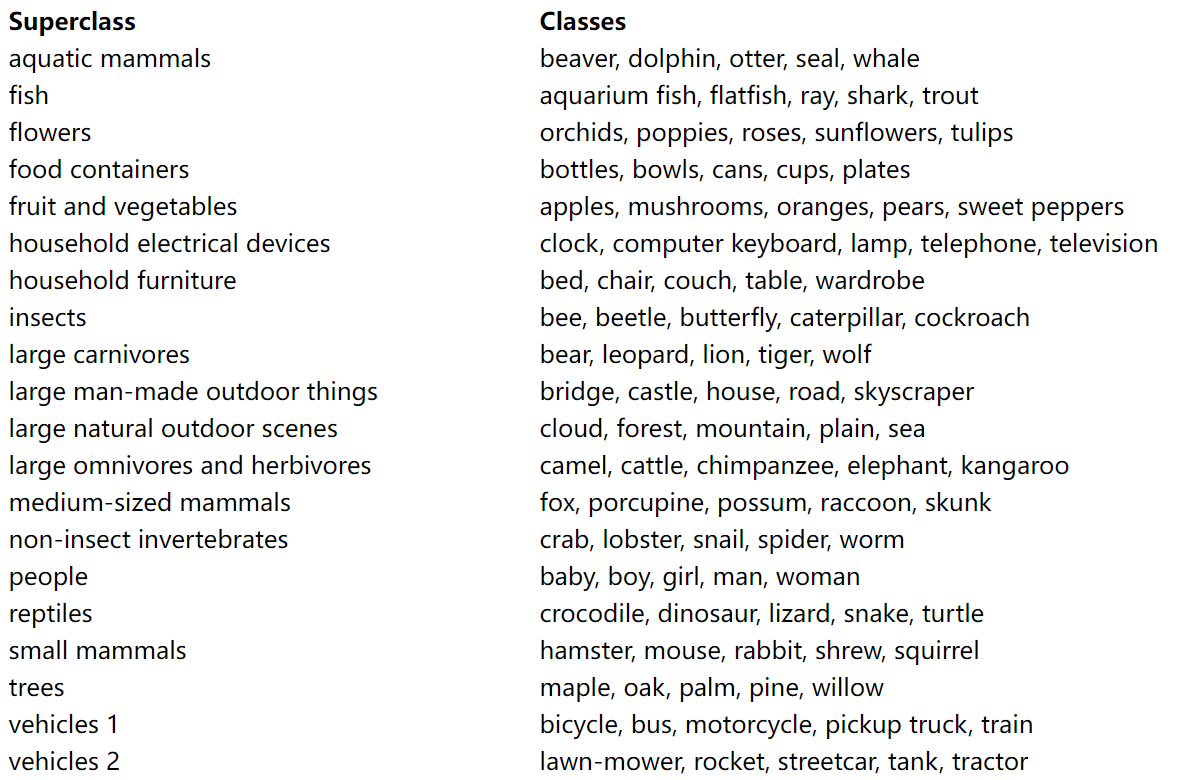
\includegraphics[width=0.90\textwidth]{../img/cifar100-classes.png}
    \caption{CIFAR-100数据集的标签}
\end{figure}

下面展示了CIFAR-100训练集中的9张图像:

\begin{figure}[htbp]
    \centering
    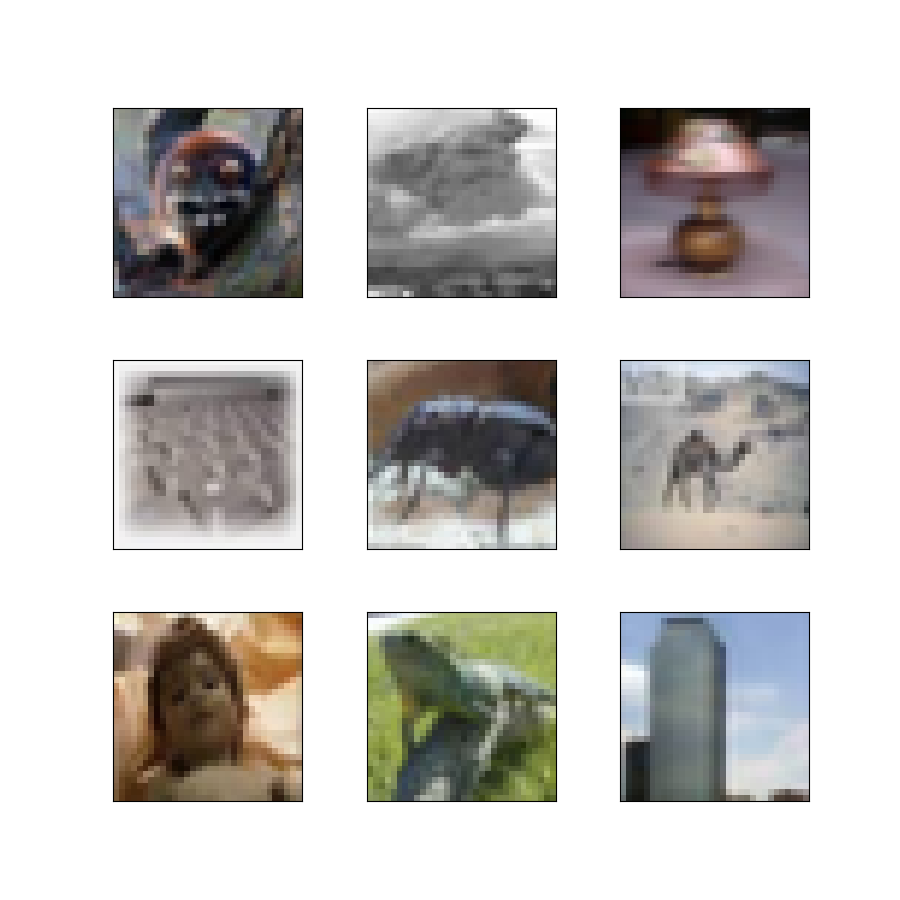
\includegraphics[width=0.30\textwidth]{../img/cifar100.png}
    \caption{CIFAR-100数据集的图像示例}
\end{figure}


\subsection{baseline模型}

\subsubsection{模型基本结构}
残差网络(ResNet)由微软研究院的何恺明、张祥雨、任少卿、孙剑等人在Deep Residual Learning for Image Recognition一文中提出,
在2015年的ILSVRC(ImageNet Large Scale Visual Recognition Challenge)中取得了冠军。
ResNet认为,理论上,可以训练一个相对浅层的网络,然后在这个训练好的相对浅层的网络上堆几层恒等映射层,
即输出等于输入的层,构建出一个更深层的网络。这两个网络得到的结果应该是一模一样的,
因而在训练集上,深层的网络不会比浅层的网络效果差。


ResNet通过加入shortcut connections,变得更加容易被优化。
包含一个shortcut connection的几层网络被称为一个残差块(residual block),如图3所示。


\begin{figure}[htbp]
    \centering
    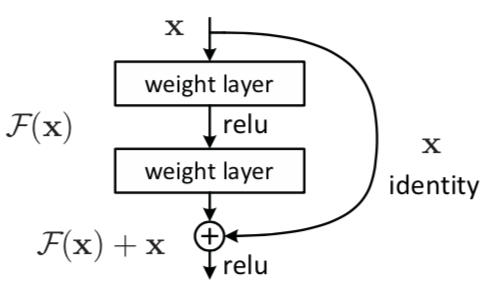
\includegraphics[width=0.40\textwidth]{../img/1-1.png}
    \caption{残差块}
\end{figure}

如图4所示,展示了ResNet的几种结构:

\begin{figure}[htbp]
    \centering
    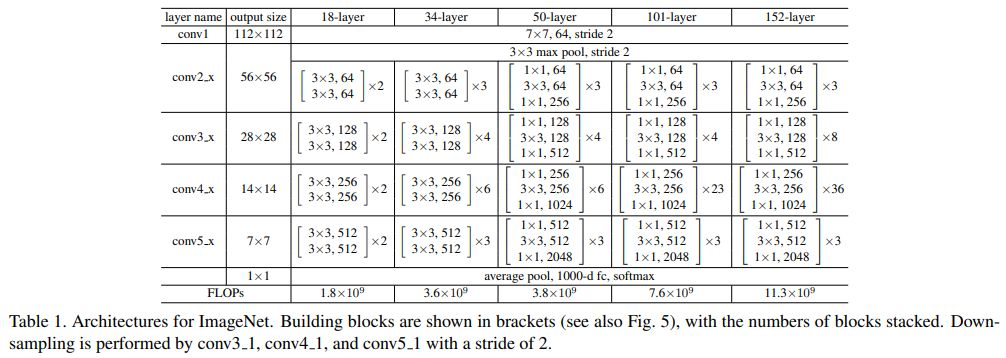
\includegraphics[width=0.90\textwidth]{../img/1-2.jpg}
    \caption{ResNet的几种结构}
\end{figure}

其中,ResNet-18和ResNet-34使用两个$3\times3$的卷积层作为一个块,
而ResNet-50,ResNet-101和ResNet-152将其替换为$1\times1+3\times3+1\times1$的卷积进行计算优化,
这样的块即减少了计算量又能够保持精度,被称为BottleNeck块。

另外,为了使得输入和输出保持相同的维度,若特征图维度不同,
对于卷积层的残差块,需要在$1\times1$卷积后添加批归一化(Batch Normalization)处理,如图5所示。

\begin{figure}[htbp]
    \centering
    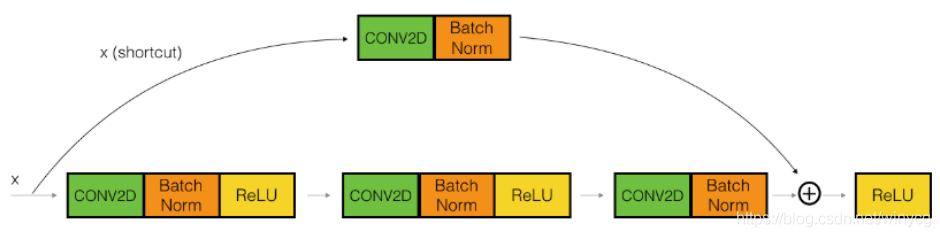
\includegraphics[width=0.90\textwidth]{../img/1-3.png}
    \caption{批归一化}
\end{figure}

考虑到训练的效率,我们使用ResNet-18作为baseline模型。由于CIFAR-100的图像较小,
ResNet-18中的第一层卷积使用$7\times7$卷积核可能过大,难以提取CIFAR-100图像的特征,
我们将其调整为$3\times3$卷积核。此外,模型的其它的baseline如下:
\begin{itemize}
    \item epoch:100
    \item batch size:100
    \item drop out:不使用
    \item 损失函数:交叉熵损失
    \item 正则化:$l_2$正则化,正则化参数$\lambda=10^{-5}$
    \item 优化器:Adam
    \item 动量系数:$\beta_1=0.9, \beta_2=0.999$
    \item 初始学习率:$\alpha=10^{-3}$
    \item 学习率衰减:每个epoch后学习率衰减为上一个epoch的0.98
\end{itemize}

我们得到baseline模型
在测试集上的平均误差为$\textbf{2.455}$,分类精度为$\textbf{0.604}$。
模型的性能曲线如下所示:

\begin{figure}[htbp]
    \centering
    \subfigure[accuracy曲线]{
        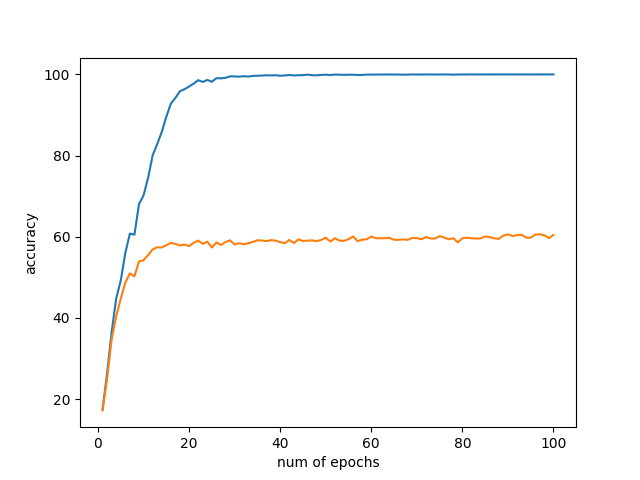
\includegraphics[width=0.40\textwidth]{../img/accuracy1.png}
    }
    \hspace{0.5in}
    \subfigure[loss曲线]{
        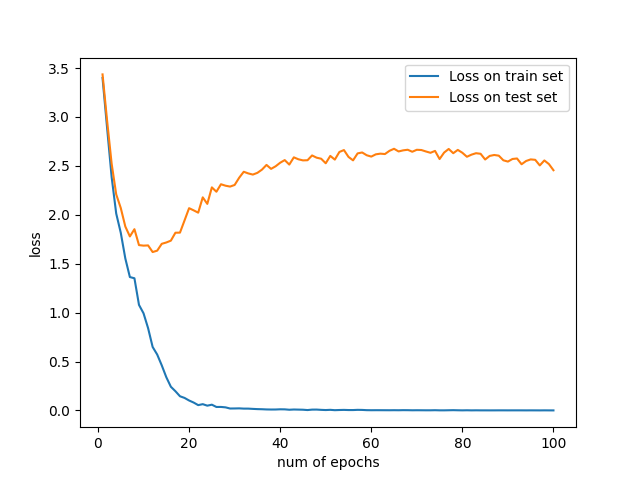
\includegraphics[width=0.40\textwidth]{../img/loss1.png}
    }
    \caption{baseline模型的性能曲线}
\end{figure}

可以发现,模型的精度较低,且模型存在较严重的振荡和过拟合现象。

\subsubsection{模型超参数调整}
为了缓解模型的过拟合现象,我们将baseline模型的超参数进行调整,
以得到较高的精度。调整后模型的超参数如下:
\begin{itemize}
    \item epoch:100
    \item batch size:100
    \item drop out:使用
    \item 损失函数:交叉熵损失
    \item 正则化:$l_2$正则化,正则化参数$\lambda=10^{-3}$
    \item 优化器:SGD
    \item 动量系数:$\beta=0.9$
    \item 初始学习率:$\alpha=10^{-2}$
    \item 学习率衰减:每个epoch后学习率衰减为上一个epoch的0.98
\end{itemize}

经过调整后,我们得到模型
在测试集上的平均误差为$\textbf{1.317}$,分类精度为$\textbf{0.672}$。
模型的性能曲线如下所示:

\begin{figure}[htbp]
    \centering
    \subfigure[accuracy曲线]{
        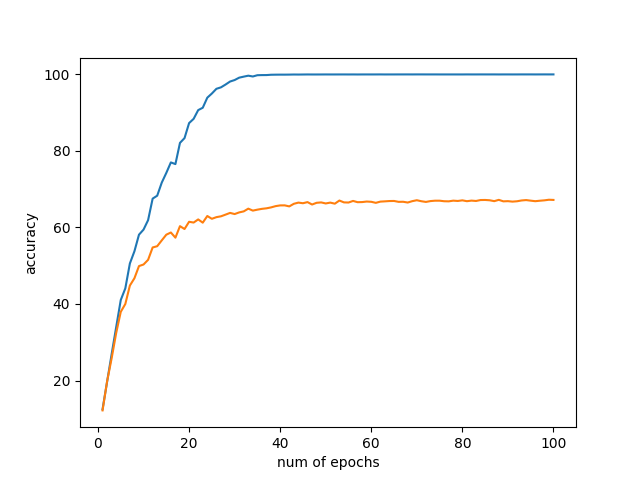
\includegraphics[width=0.40\textwidth]{../img/accuracy2.png}
    }
    \hspace{0.5in}
    \subfigure[loss曲线]{
        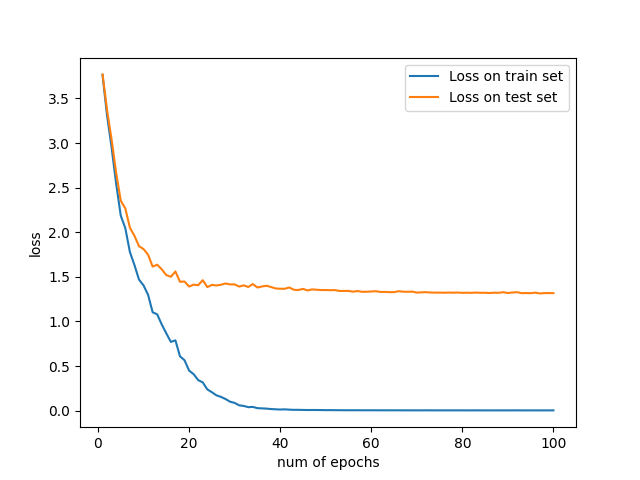
\includegraphics[width=0.40\textwidth]{../img/loss2.png}
    }
    \caption{调整后的性能曲线}
\end{figure}

可以发现,模型的过拟合现象得到了一定程度的改善,精度得到了提高,
且不再出现测试集上loss随训练过程增加的现象。

\subsection{数据增强}
由于数据增强后,模型较难学习到图像的特征,
因此我们调整训练的epoch数至200个,且调整学习率衰减系数至0.98。

\subsubsection{随机裁剪和水平翻转}
我们可以对模型的数据作一些简单的数据增强。
基于torchvision自带的transforms.RandomCrop和
transforms.RandomHorizontalFlip函数,
我们可以简单地实现对训练集图像进行向四周填充后随机裁剪以及随机翻转的操作。
这两种操作不会对图像的基本信息造成太大影响。

\begin{figure}[htbp]
    \centering
    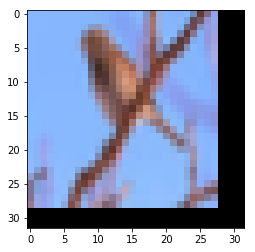
\includegraphics[width=0.20\textwidth]{../img/1-4.png}
    \caption{向四周填充后随机裁剪的效果}
\end{figure}

经过随机裁剪和水平翻转后,我们得到模型
在测试集上的平均误差为$\textbf{1.090}$,分类精度为$\textbf{0.740}$。
模型的性能曲线如下所示:

\begin{figure}[htbp]
    \centering
    \subfigure[accuracy曲线]{
        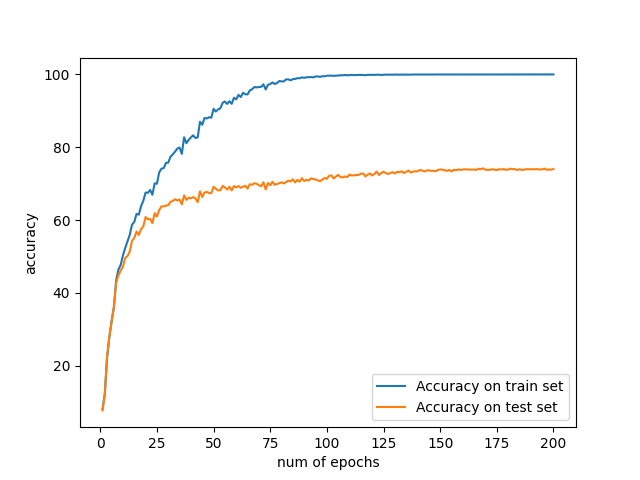
\includegraphics[width=0.40\textwidth]{../img/accuracy3.png}
    }
    \hspace{0.5in}
    \subfigure[loss曲线]{
        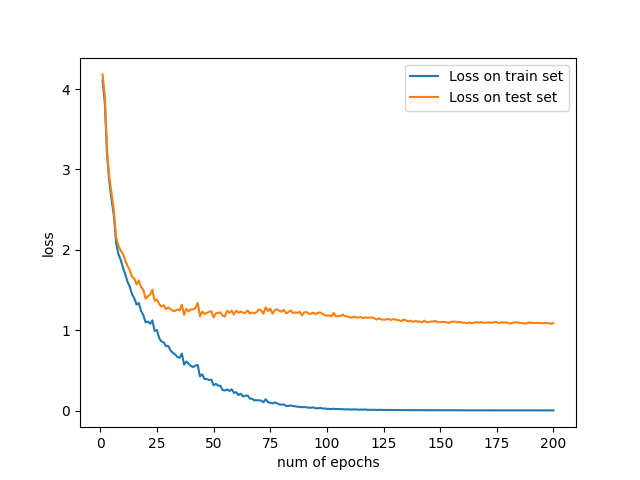
\includegraphics[width=0.40\textwidth]{../img/loss3.png}
    }
    \caption{增强后模型的性能曲线}
\end{figure}

\subsubsection{Cut out}
Cut out的原理是:随机将样本中的部分区域去掉,
然后填充0像素值,分类的结果不变。
下面展示了三张训练集样本Cut out后的图像:

\begin{figure}[htbp]
    \centering
    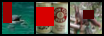
\includegraphics[width=0.40\textwidth]{../img/sample_cutout.png}
    \caption{cutout的效果}
\end{figure}

基于torchtoolbox包自带的Cutout方法,我们在数据增强时增加Cut out操作,
设置对图像进行Cutout的概率为0.5。进行Cut out后,
得到模型在测试集上的平均误差为$\textbf{1.076}$,分类精度为$\textbf{0.729}$。
模型的性能曲线如图11所示:

\begin{figure}[htbp]
    \centering
    \subfigure[accuracy曲线]{
        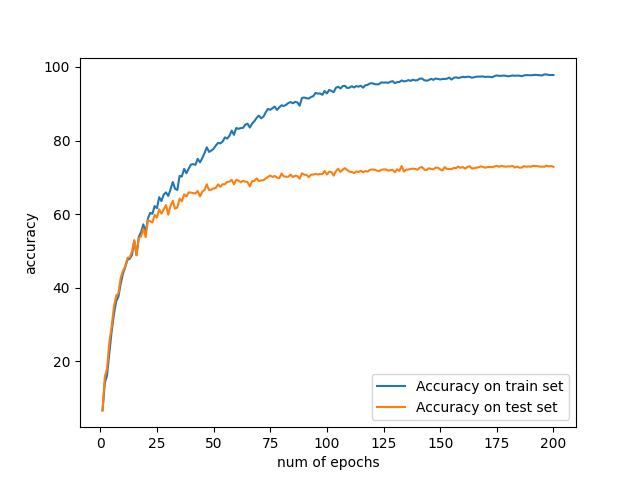
\includegraphics[width=0.40\textwidth]{../img/accuracy4.png}
    }
    \hspace{0.5in}
    \subfigure[loss曲线]{
        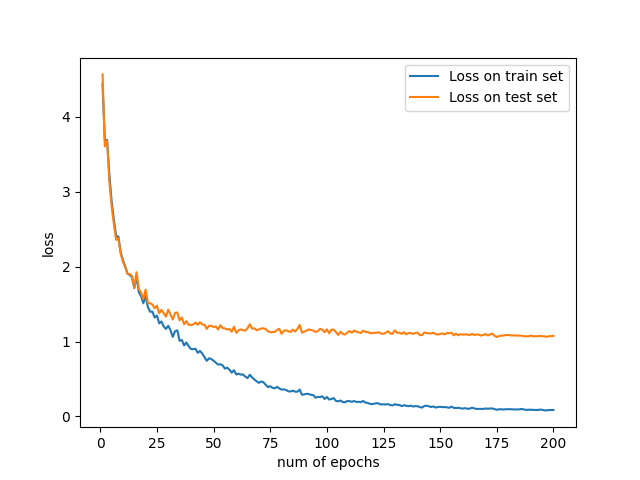
\includegraphics[width=0.40\textwidth]{../img/loss4.png}
    }
    \caption{cutout后模型的性能曲线}
\end{figure}

我们可以可视化五个中间block各一个特征通道的输出,如图12所示:

\begin{figure}[h]
    \centering
    \subfigure[输入层]{
        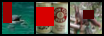
\includegraphics[width=0.20\textwidth]{../img/sample_cutout.png}
    }
    \hspace{0.5in}
    \subfigure[Conv1层输出]{
        
\includegraphics[width=0.20\textwidth]{../img/sample_cutouthidden1.png}
    }
    \hspace{0.5in}
    \subfigure[Conv2层输出]{
        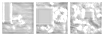
\includegraphics[width=0.20\textwidth]{../img/sample_cutouthidden2.png}
    }
    \hspace{0.5in}
    \subfigure[Conv3层输出]{
        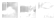
\includegraphics[width=0.20\textwidth]{../img/sample_cutouthidden3.png}
    }
    \hspace{0.5in}
    \subfigure[Conv4层输出]{
        
\includegraphics[width=0.20\textwidth]{../img/sample_cutouthidden4.png}
    }
    \hspace{0.5in}
    \subfigure[Conv5层输出]{
        
\includegraphics[width=0.20\textwidth]{../img/sample_cutouthidden5.png}
    }
    \caption{隐藏层输出可视化}
\end{figure}

\subsubsection{Cutmix}
Cutmix的原理是:将一部分区域去掉,但不是填充随机的固定像素值,
而是随机填充训练集中的其他数据的区域像素值,分类结果按一定的比例分配。

Cutmix可以用公式表示:
$$\begin{aligned}
    \tilde{x} &= \textbf{M} \odot x_A + (\textbf{1}-\textbf{M}) \odot x_B \\
    \tilde{y} &= \lambda y_A + (1-\lambda) y_B
\end{aligned}$$
其中$\lambda\sim Beta(\alpha, \alpha)$,
$\textbf{M}\in\{0,1\}^{W\times H}$表示选择来自哪张图片的掩码,
$\odot$表示逐元素相乘。为此,我们还需要确定一个随机采样得到的bounding box,即
$B=(r_x,r_y,r_w,r_h)$,采样方法为:
$$\begin{aligned}
    & r_x \sim {\rm Unif}(0, W), & \quad r_w=W\sqrt{1-\lambda} \\
    & r_y \sim {\rm Unif}(0, H), & \quad r_h=H\sqrt{1-\lambda}
\end{aligned}$$
这样即可保证裁剪区域的大小为原图像的$1-\lambda$倍。

我们取$\alpha=1$,此时$\lambda\sim{\rm Unif}(0, 1)$。
图13展示了以三张训练集样本作为一个batch,经过cutmix后的图像:

\begin{figure}[htbp]
    \centering
    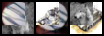
\includegraphics[width=0.40\textwidth]{../img/sample_cutmix.png}
    \caption{cutmix的效果}
\end{figure}

进行cutmix后,我们得到模型
在测试集上的平均误差为$\textbf{0.916}$,分类精度为$\textbf{0.759}$。
模型的性能曲线如图14所示:

\begin{figure}[htbp]
    \centering
    \subfigure[accuracy曲线]{
        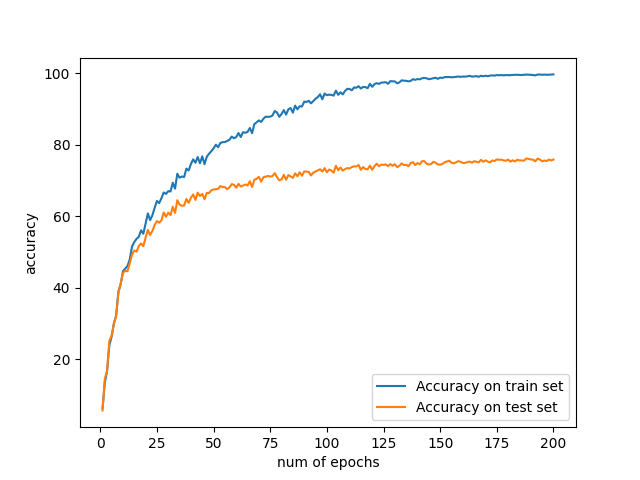
\includegraphics[width=0.40\textwidth]{../img/accuracy5.png}
    }
    \hspace{0.5in}
    \subfigure[loss曲线]{
        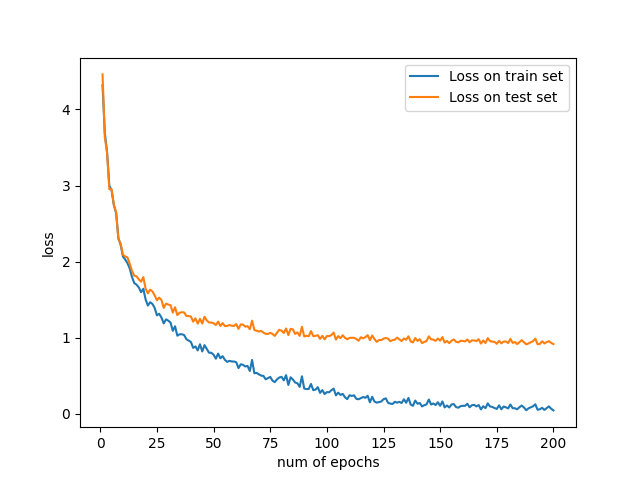
\includegraphics[width=0.40\textwidth]{../img/loss5.png}
    }
    \caption{cutmix后模型的性能曲线}
\end{figure}

可视化五个中间block各一个特征通道的输出,如图15所示。

\begin{figure}[h]
    \centering
    \subfigure[输入层]{
        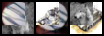
\includegraphics[width=0.20\textwidth]{../img/sample_cutmix.png}
    }
    \hspace{0.5in}
    \subfigure[Conv1层输出]{
        
\includegraphics[width=0.20\textwidth]{../img/sample_cutmixhidden1.png}
    }
    \hspace{0.5in}
    \subfigure[Conv2层输出]{
        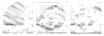
\includegraphics[width=0.20\textwidth]{../img/sample_cutmixhidden2.png}
    }
    \hspace{0.5in}
    \subfigure[Conv3层输出]{
        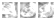
\includegraphics[width=0.20\textwidth]{../img/sample_cutmixhidden3.png}
    }
    \hspace{0.5in}
    \subfigure[Conv4层输出]{
        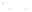
\includegraphics[width=0.20\textwidth]{../img/sample_cutmixhidden4.png}
    }
    \hspace{0.5in}
    \subfigure[Conv5层输出]{
        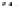
\includegraphics[width=0.20\textwidth]{../img/sample_cutmixhidden5.png}
    }
    \caption{隐藏层输出可视化}
\end{figure}

\subsubsection{Mix up}
Mixup的原理是:将两张图按比例进行插值来混合样本。

Mixup可以用公式表示:
$$\begin{aligned}
    \tilde{x} &= \lambda x_A + (1-\lambda) x_B \\
    \tilde{y} &= \lambda y_A + (1-\lambda) y_B
\end{aligned}$$
其中$\lambda\sim Beta(\alpha, \alpha)$

我们取$\alpha=0.2$,如图16所示,
展示了以三张训练集样本作为一个batch,经过Mix up后的图像。

\begin{figure}[htbp]
    \centering
    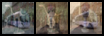
\includegraphics[width=0.40\textwidth]{../img/sample_mixup.png}
    \caption{mixup的效果}
\end{figure}

进行mixup后,我们得到模型
在测试集上的平均误差为$\textbf{1.012}$,分类精度为$\textbf{0.751}$。
模型的性能曲线如图17所示:

\begin{figure}[htbp]
    \centering
    \subfigure[accuracy曲线]{
        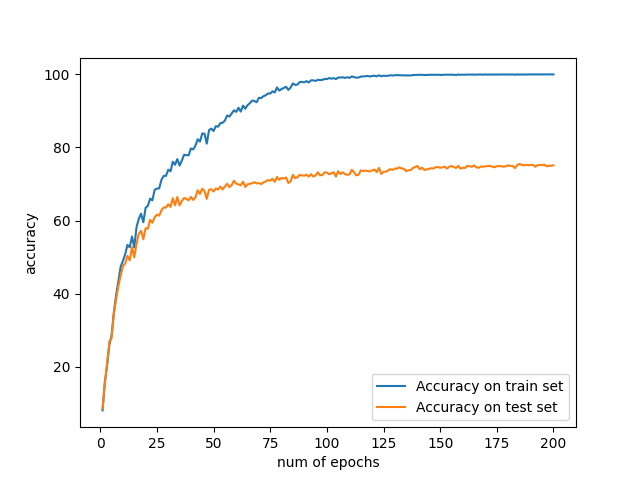
\includegraphics[width=0.40\textwidth]{../img/accuracy6.png}
    }
    \hspace{0.5in}
    \subfigure[loss曲线]{
        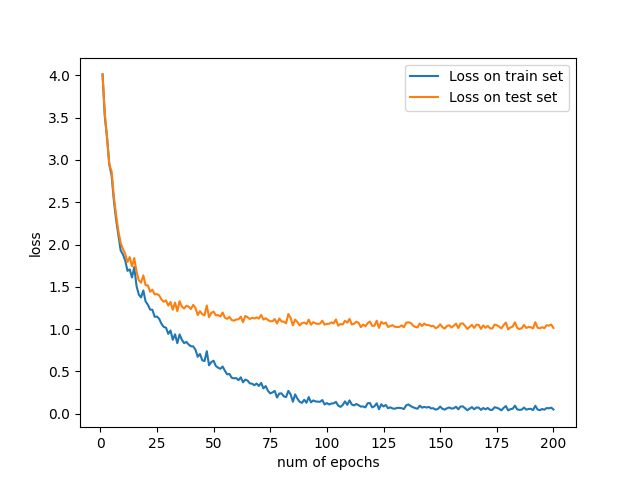
\includegraphics[width=0.40\textwidth]{../img/loss6.png}
    }
    \caption{mixup后模型的性能曲线}
\end{figure}

可视化五个中间block各一个特征通道的输出,如图18所示。

\begin{figure}[h]
    \centering
    \subfigure[输入层]{
        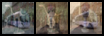
\includegraphics[width=0.20\textwidth]{../img/sample_mixup.png}
    }
    \hspace{0.5in}
    \subfigure[Conv1层输出]{
        
\includegraphics[width=0.20\textwidth]{../img/sample_mixuphidden1.png}
    }
    \hspace{0.5in}
    \subfigure[Conv2层输出]{
        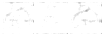
\includegraphics[width=0.20\textwidth]{../img/sample_mixuphidden2.png}
    }
    \hspace{0.5in}
    \subfigure[Conv3层输出]{
        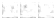
\includegraphics[width=0.20\textwidth]{../img/sample_mixuphidden3.png}
    }
    \hspace{0.5in}
    \subfigure[Conv4层输出]{
        
\includegraphics[width=0.20\textwidth]{../img/sample_mixuphidden4.png}
    }
    \hspace{0.5in}
    \subfigure[Conv5层输出]{
        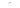
\includegraphics[width=0.20\textwidth]{../img/sample_mixuphidden5.png}
    }
    \caption{隐藏层输出可视化}
\end{figure}

\subsection{小结}
我们总共得出下面四个模型:
\begin{itemize}
    \item baseline模型(ResNet-18,经过超参数调整)
    \item baseline模型 + cutout
    \item baseline模型 + cutmix
    \item baseline模型 + mixup
\end{itemize}

四个模型在测试集上的loss和accurary如下表所示:

\begin{table}[!ht]
    \begin{center}
        \begin{tabular}{ccc}
            \hline
            模型  & 测试集误差 & 测试集精度 \\ \hline
            baseline & 1.040 & 74.0\% \\ \hline
            baseline + cutout & 1.076 & 72.9\% \\ \hline
            baseline + cutmix & 0.916 & 75.9\% \\ \hline
            baseline + mixup & 1.012 & 75.1\% \\ \hline
            \end{tabular}
        \caption{不同数据增强方式对模型性能的影响}
    \end{center}
\end{table}

我们发现,在baseline模型上,增加cutmix方法对数据进行增强,
相对于cutout和mixup两种方法达到的测试集上的误差最小,精度最高。
可以总结出cutmix的以下几个优点:
\begin{itemize}
    \item 在训练过程中不会出现非信息像素,从而能够提高训练效率;
    \item 保留了cutout方法regional dropout的优势,能够关注目标的non-discriminative parts;
    \item 通过要求模型从局部视图识别对象,对cut区域中添加其他样本的信息,能够进一步增强模型的定位能力;
    \item 相较于mixup方法,不会有图像混合后不自然的情形,能够提升模型分类的表现;
    \item 训练和推理的代价保持不变。
\end{itemize}

\newpage
\section{在VOC数据集上训练Faster R-CNN和YOLO V3}
\subsection{数据集介绍与划分}

\subsubsection{数据集总体概况}
PASCAL对于目标检测或分割类型来说属于先驱者的地位。
对于现在的研究者来说比较重要的两个年份的数据集是 $\textbf{PASCAL VOC 2007}$ 
与 $\textbf{PASCAL VOC 2012}$,
这两个数据集频频在现在的一些检测或分割类的论文当中出现。

由于从2007年之后,PASCAL VOC的测试集均不再公布,
因此我们选择PASCAL VOC 2007作为我们的数据集。
下面展示了PASCAL VOC 2007数据集的20个类别及其层级结构:
\begin{figure}[htbp]
    \centering
    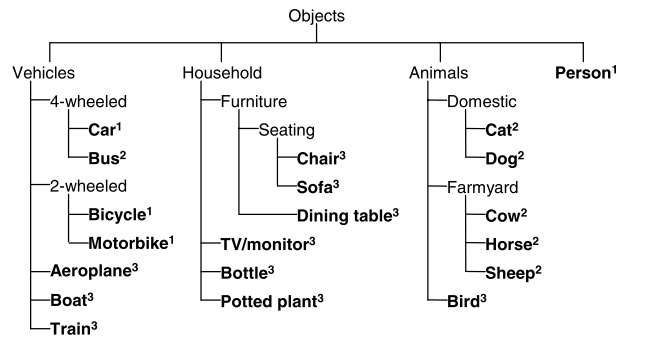
\includegraphics[width=0.90\textwidth]{../img/VOC2007-classes.png}
    \caption{VOC 2007数据集的标签}
\end{figure}

其中:
\begin{itemize}
    \item 分为4个大类,20个小类。预测时主要输出的小类。
    \item 数据集主要关注分类和检测,也就是分类和检测用到的数据集相对规模较大。关于其他任务比如分割,动作识别等,其数据集一般是分类和检测数据集的子集。
\end{itemize}

如图20所示,展示了PASCAL VOC 2007数据集总体的统计情况。
\begin{figure}[htbp]
    \centering
    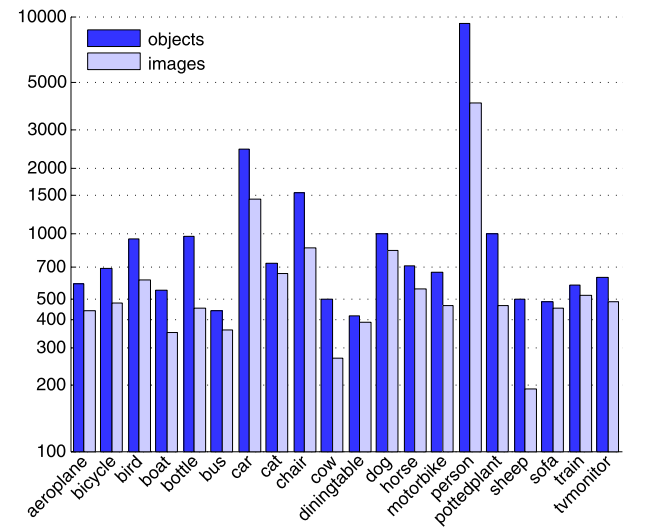
\includegraphics[width=0.60\textwidth]{../img/VOC2007-histogram.png}
    \caption{VOC 2007数据集的统计情况}
\end{figure}

\subsubsection{数据集划分}
PASCAL VOC 2007数据集分为两部分:训练和验证集trainval,测试集test,
两部分各占数据总量的约 50\%。
其中trainval又分为训练集和测试集,二者分别各占trainval的50\%。
每张图片中有可能包含不只一个目标object。

如图21所示,展示了数据集在训练集,验证集,测试集上的划分情况。
\begin{figure}[htbp]
    \centering
    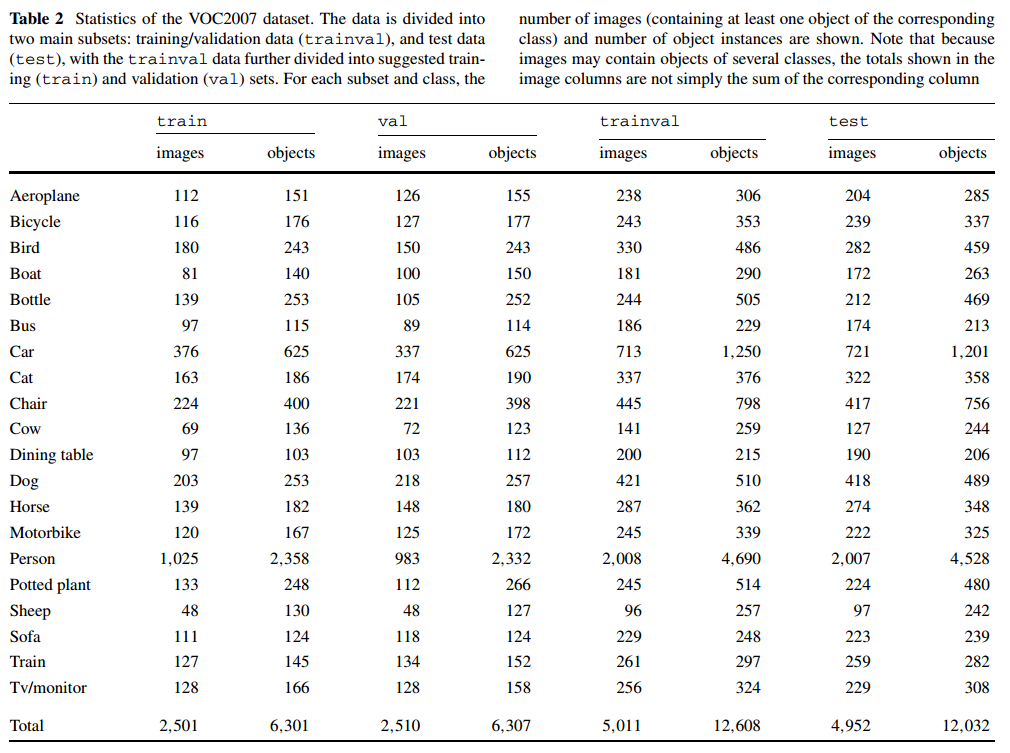
\includegraphics[width=1.00\textwidth]{../img/VOC2007-stats.png}
    \caption{VOC 2007数据集的具体划分情况}
\end{figure}

\subsubsection{数据集可视化}
\url{http://host.robots.ox.ac.uk/pascal/VOC/voc2007/examples/index.html}

网站中展示了VOC-2007中至少包含每个类一个目标的8张图像及其目标的ground truth位置。
下面展示一部分:
\begin{figure}[h]
    \centering
    \subfigure[Aeroplanes]{
        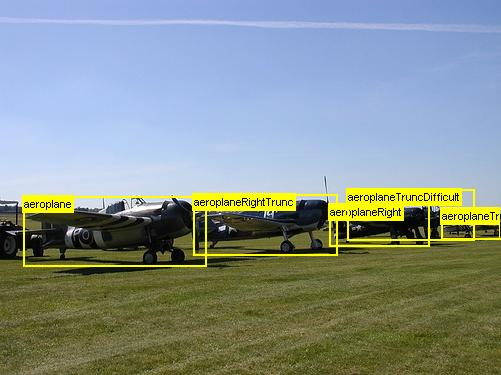
\includegraphics[width=0.40\textwidth]{../img/VOC2007-sample1.jpg}
    }
    \hspace{0.5in}
    \subfigure[Bicycles]{
        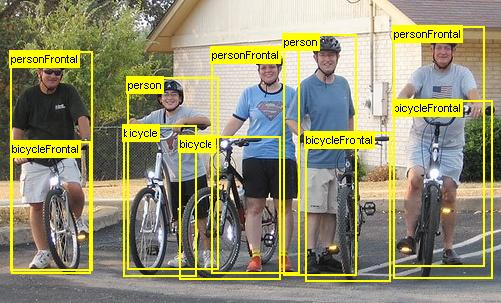
\includegraphics[width=0.40\textwidth]{../img/VOC2007-sample2.jpg}
    }
    \hspace{0.5in}
    \subfigure[Birds]{
        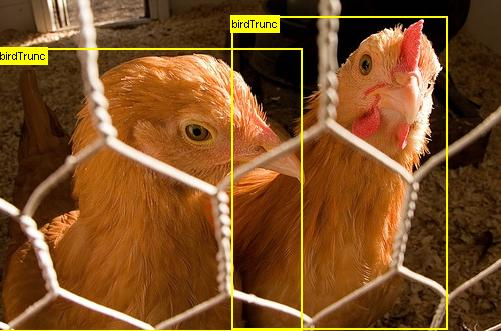
\includegraphics[width=0.40\textwidth]{../img/VOC2007-sample3.jpg}
    }
    \hspace{0.5in}
    \subfigure[Boats]{
        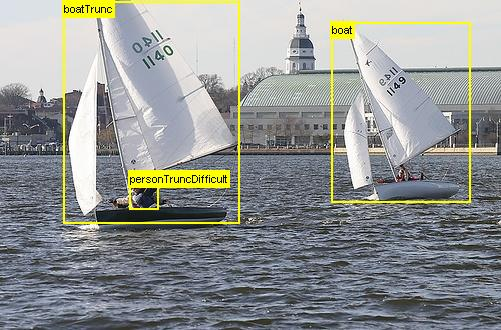
\includegraphics[width=0.40\textwidth]{../img/VOC2007-sample4.jpg}
    }
    \hspace{0.5in}
    \subfigure[Bottles]{
        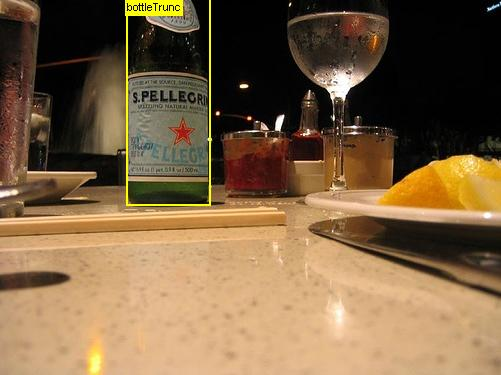
\includegraphics[width=0.40\textwidth]{../img/VOC2007-sample5.jpg}
    }
    \hspace{0.5in}
    \subfigure[Buses]{
        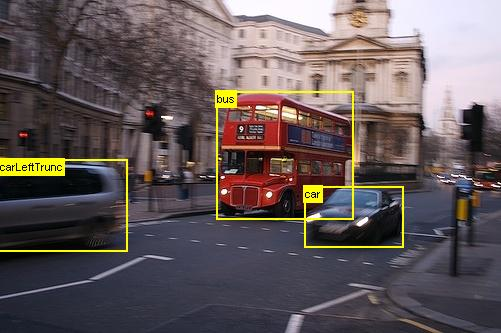
\includegraphics[width=0.40\textwidth]{../img/VOC2007-sample6.jpg}
    }
    \caption{VOC 2007数据集示例}
\end{figure}

\subsubsection{读取VOC数据集}
使用torchvision.datasets包中的VOCDetection下载数据集,在VOC2007文件夹中,得到下面几个部分:
\begin{itemize}
    \item Annotations:包含了记录图像和标签信息的xml文件
    \item ImageSets:主要包含划分的训练集和测试集中图片的名称
    \item JPEGImages:包含数据集的原始图片
    \item SegmentationClass:按类别分割的ground truth位置
    \item SegmentationObject:按对象分割的ground truth位置
\end{itemize}

我们读取了四张训练集的图像并对其目标的ground truth进行了标注:
\begin{figure}[h]
    \centering
    \subfigure[图片1]{
        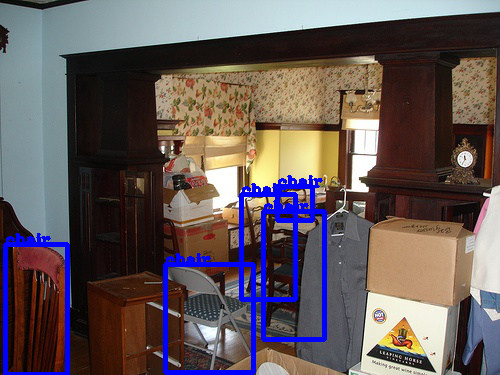
\includegraphics[width=0.40\textwidth]{../img/image_0.png}
    }
    \hspace{0.5in}
    \subfigure[图片2]{
        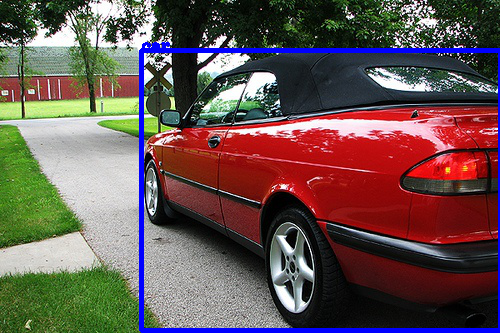
\includegraphics[width=0.40\textwidth]{../img/image_1.png}
    }
    \hspace{0.5in}
    \subfigure[图片3]{
        \includegraphics[width=0.40\textwidth]{../img/image_2.png}
    }
    \hspace{0.5in}
    \subfigure[图片4]{
        \includegraphics[width=0.40\textwidth]{../img/image_3.png}
    }
    \caption{VOC 2007训练集图像ground truth标注示例}
\end{figure}

\subsection{Faster R-CNN模型}
\subsubsection{基本结构}
经过R-CNN和Fast R-CNN的积淀,Ross B. Girshick在2016年提出了新的Faster R-CNN,
在结构上,Faster R-CNN已经将特征抽取(feature extraction),proposal提取,
bounding box regression(rect refine),classification都整合在了一个网络中,
使得综合性能有较大提高,在检测速度方面尤为明显。

整个Faster R-CNN分为4大部分:
共享卷积网络,候选检测框生成网络RPN(Region Proposal Networks),
感兴趣区域池化RoI(Region of Interest)Pooling和分类器。
如图24所示。

\begin{figure}[htbp]
    \centering
    \includegraphics[width=0.50\textwidth]{../img/fasterR-CNN.jpg}
    \caption{Faster R-CNN基本结构}
\end{figure}

其中:
\begin{itemize}
    \item 共享卷积网络(Conv layers):提取image的feature maps。
    该feature maps被共享用于后续RPN层和全连接层。
    \item 候选检测框生成网络(RPN):RPN网络用于生成region proposals。该层通过softmax判断anchors
    属于positive或者negative,再利用bounding box regression
    修正anchors获得精确的proposals。
    \item 感兴趣区域池化(RoI Pooling):该层收集输入的feature maps和proposals,
    综合这些信息后提取proposal feature maps,送入后续全连接层判定目标类别。
    \item 分类器(classifier):利用proposal feature maps计算proposal的类别,
    同时再次bounding box regression获得检测框最终的精确位置。
\end{itemize}

\subsubsection{模型训练}

\subsubsection{模型评价}

\subsubsection{模型可视化}

\subsection{YOLO V3模型}


\end{document}